% Schematic representation of mach zender interferometer
% Modified from a version created by Henrik Kröger, https://github.com/derhedwig/fiberoptics/blob/master/auswertung.tex
% Author: Orlando Torres (2016)

\documentclass{standalone}
\usepackage{amsmath} % Required for \varPsi below
\usepackage{tikz,pgfplots}
\usetikzlibrary{calc}
\usetikzlibrary{patterns}

\begin{document}
  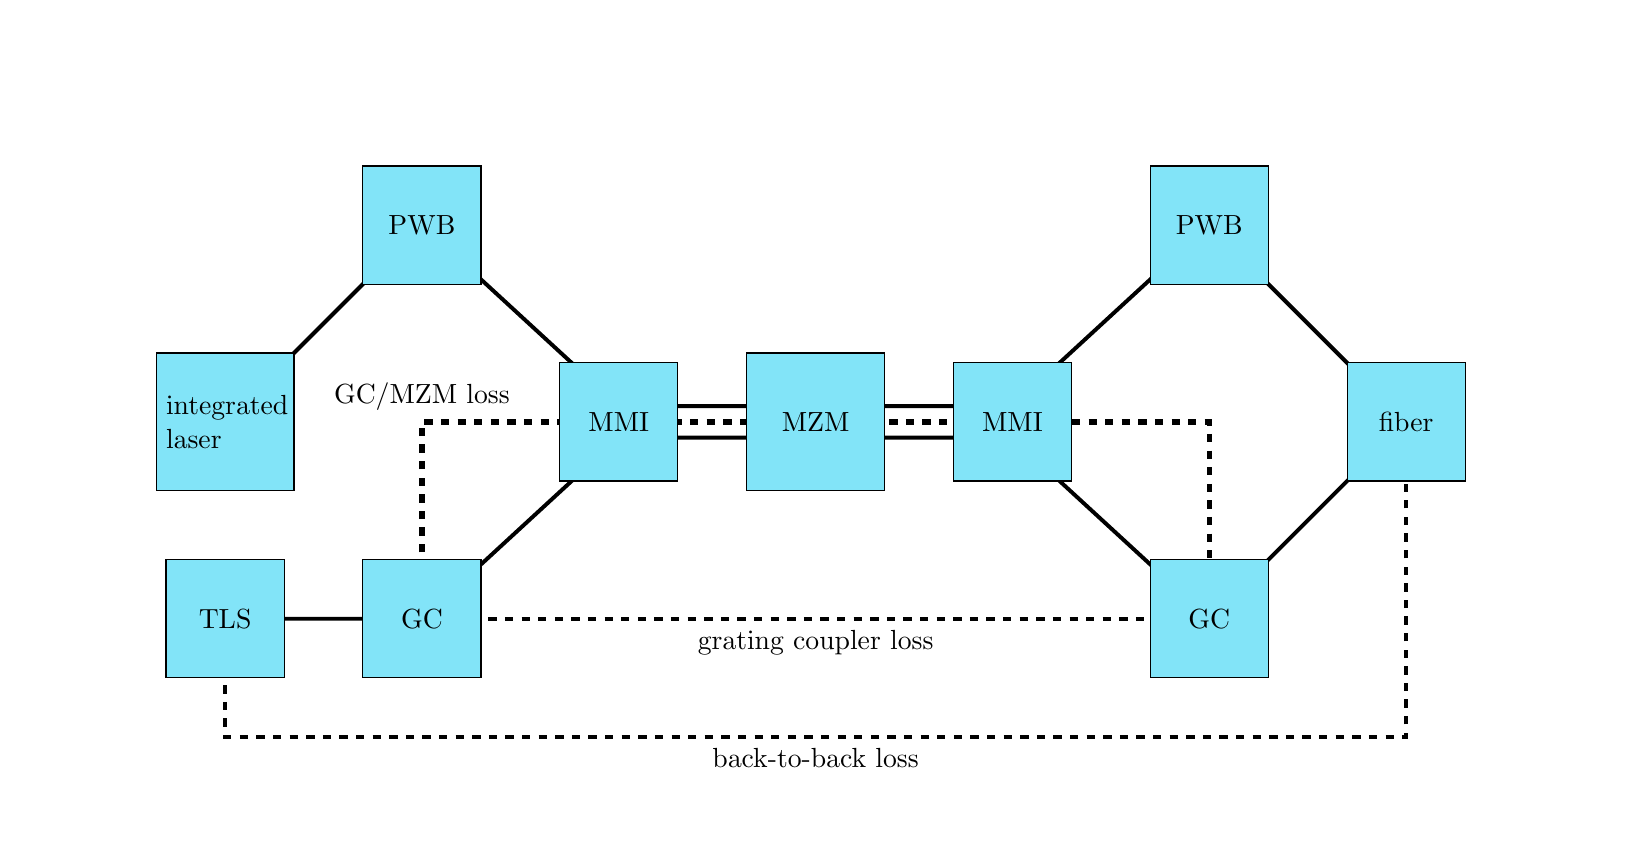
\begin{tikzpicture}
   	%define colors
    \definecolor{bbblue}{rgb}{0.964, 0.866, 0.474}
    \definecolor{rrred}{rgb}{0.952, 0.815, 0.105}
    \definecolor{yyyellow}{rgb}{0.925, 0.827, 0.152}    
    %0.933, 0.756, 0.227
    \definecolor{lblue}{rgb}{0.509, 0.894, 0.972}
    \definecolor{sblue}{rgb}{0.607, 0.733, 0.929}
	\definecolor{lyel}{rgb}{0.925, 0.827, 0.152}
    
    %define coordinates for laser integrated
	\coordinate (laser) at (-75.0mm, 0);
	 %define coordinates for laser
	\coordinate (laserext) at (-75.0mm, -25mm);
    %define coordinates for pwb
	\coordinate (pwbi) at (-50.0mm, +25.0mm);
	%define coordinates for grating coupler
	\coordinate (gci) at (-50.0mm, -25.0mm);
	%define coordinates for mmi
	\coordinate (mmii) at (-25.0mm, 0);
	%define coordinates for grating coupler
	\coordinate (MZM) at (0, 0);
	%define coordinates for mmi
	\coordinate (mmio) at (+25.0mm, 0);
	%define coordinates for mmi
	\coordinate (gco) at (+50.0mm, -25.0mm);
    %define coordinates for pwb
	\coordinate (pwbo) at (+50.0mm, +25.0mm);	
    %define coordinates for fiber
	\coordinate (fiber) at (+75.0mm, 0);

    % Substrate, modulators, Waveguides, MMI and converters %    
    \node [shape=rectangle, minimum width=200mm, minimum height=100mm, color=white, draw,fill=white]
    (substrate) at (0,0) {};  

    % Optical path %
    \draw  [line width=0.5mm, color=black] (laser) -- (pwbi) -- ($(mmii)+(0mm, 2mm)$) -- ($(MZM)+(0mm, 2mm)$) -- ($(mmio)+(0mm, 2mm)$) -- (pwbo) -- (fiber);
    \draw  [line width=0.5mm, color=black] (laserext) -- (gci) -- ($(mmii)+(0mm, -2mm)$) -- ($(MZM)+(0mm, -2mm)$) -- ($(mmio)+(0mm, -2mm)$) -- (gco) -- (fiber);
    
    %back-to-back link
    \draw  [line width=0.5mm, color=black,dashed] (laserext) -- ($(laser)+(0mm, -40mm)$) -- ($(MZM)+(0mm, -40mm)$) node[below] {back-to-back loss} -- ($(fiber)+(0mm, -40mm)$) -- (fiber);
    %\draw  [line width=0.5mm, color=red] (laserext) -- ($(laser)+(0mm, -40mm)$) -- ($(MZM)+(0mm, -40mm)$) node[below] {back-to-back loss} -- ($(fiber)+(0mm, -40mm)$) -- (fiber);
    \draw  [line width=0.5mm, color=black,dashed] (gci) -- ($(MZM)+(0mm, -25mm)$) node[below] {grating coupler loss} -- (gco);
	\draw  [line width=0.7mm, color=black,dashed] (gci) -- ($(gci)+(0mm, +25mm)$) node[above] {GC/MZM loss}  --  ($(MZM)+(0mm, +0mm)$)  --($(gco)+(0mm, +25mm)$) -- (gco);
	%\draw  [line width=0.7mm, color=red] (laserext) -- (gci);
	%\draw  [line width=0.7mm, color=red] (gco) -- (fiber);
    %PWB
    %\draw [line width=1.20mm,red] plot [smooth, tension=1] coordinates {($ (pwbi) + (-2mm, 0mm) $)  ($ (gci) + (1mm, 1mm) $) ($ (gco) + (5mm, 5mm) $) ($ (MZM) + (-3mm, 1mm) $) ($ (fiber) + (2mm, 0mm) $)};
    
    %\draw [fill=orange] (lasersubs) rectangle (0.2,0.2); 
    \node [shape=rectangle, minimum width=17.5mm, minimum height=17.5mm, color=black, fill=lblue, draw]
    (lasers) at (laser) {}; 
     \node [shape=rectangle, minimum width=15mm, minimum height=15mm, color=black, fill=lblue, draw]
    (laserse) at (laserext) {TLS}; 
    \node [shape=rectangle, minimum width=15mm, minimum height=15mm, color=black, fill=lblue, draw]
    (pwbis) at (pwbi) {PWB}; 
    \node [shape=rectangle, minimum width=15mm, minimum height=15mm, color=black, fill=lblue, draw]
    (gcis) at (gci) {GC}; 
    \node [shape=rectangle, minimum width=15mm, minimum height=15mm, color=black, fill=lblue, draw]
    (mmiis) at (mmii) {MMI}; 
    \node [shape=rectangle, minimum width=17.5mm, minimum height=17.5mm, color=black, fill=lblue, draw]
    (MZMs) at (MZM) {MZM}; 
    \node [shape=rectangle, minimum width=15mm, minimum height=15mm, color=black, fill=lblue, draw]
    (mmios) at (mmio) {MMI}; 
    \node [shape=rectangle, minimum width=15mm, minimum height=15mm, color=black, fill=lblue, draw]
    (gcos) at (gco) {GC}; 
    \node [shape=rectangle, minimum width=15mm, minimum height=15mm, color=black, fill=lblue, draw]
    (pwbos) at (pwbo) {PWB}; 
    \node [shape=rectangle, minimum width=15mm, minimum height=15mm, color=black, fill=lblue, draw]
    (fibs) at (fiber) {fiber}; 
    
    \draw (lasers) node [text width=10mm] (laser) at ($(laser)+(-2.5mm, 0mm)$) {integrated \\ laser};
    
  \end{tikzpicture}
\end{document}